\documentclass{jarticle}
\usepackage{style}
\usepackage{fancyheadings}
\usepackage[dvipdfmx]{color}
\usepackage[dvipdfmx]{graphicx}
\usepackage{color}
\usepackage{amsmath}
\usepackage{algorithmic}
\usepackage[hyphens]{url}
\usepackage{txfonts}
\usepackage{listings}

\newcommand{\tref}[1]{表~\ref{#1}}
\newcommand{\eref}[1]{(\ref{#1})~式}
\newcommand{\fref}[1]{図~\ref{#1}}
\newcommand{\sref}[1]{リスト~\ref{#1}}
\renewcommand{\lstlistingname}{リスト}

\jtitle{Title}
\etitle{Title Eng}
\jauthor{author}
\eauthor{Author Eng}
\englishabstract{Abst Eng}

\begin{document}

\maketitle

\section{はじめに}
  template template template template template template template template template template \\
  template template template template template template template template template template \\
  template template template template template template template template template template
  \begin{figure}[htbp]
    \begin{center}
      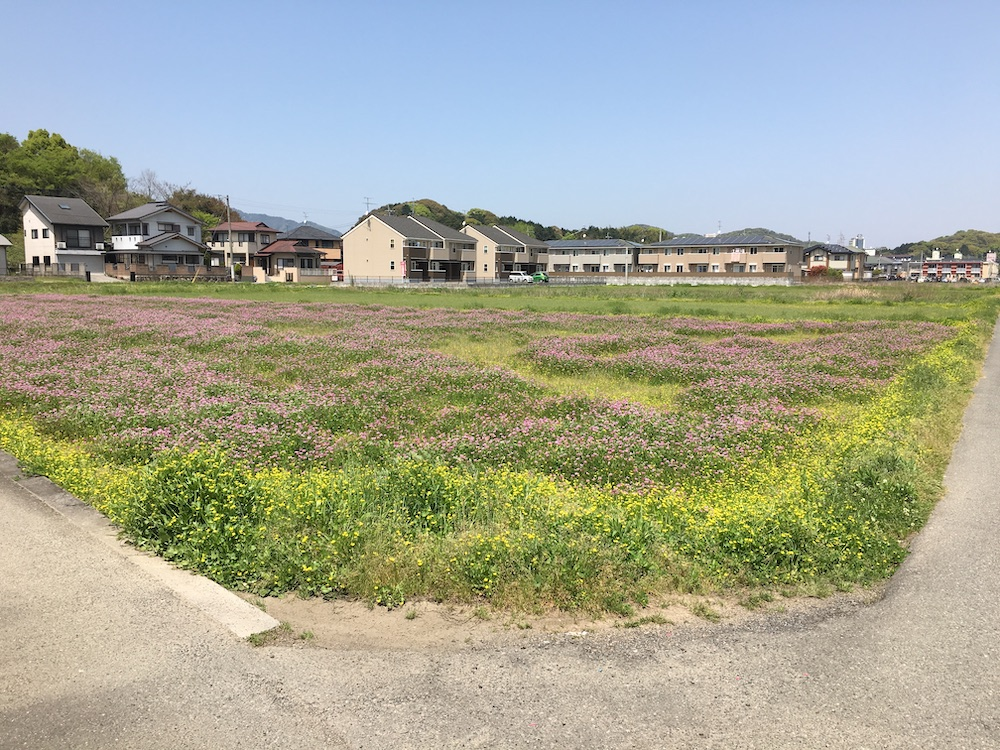
\includegraphics[width=0.9\linewidth]{images/template.jpg}
      \vspace*{-0.3cm}
      \caption{image caption}
      \label{fig:template}
    \end{center}
  \end{figure}


\section{次に}
template template template template template template template template template template \\
template template template template template template template template template template \\
template template template template template template template template template template

\section{テーブルスニペット}
template template template template template template template template template template \\
template template template template template template template template template template \\
template template template template template template template template template template
  \begin{table}[htbp]
    \begin{center}
      \caption{caption}
      \begin{tabular}{|l|l|l|} \hline
        A & 1 \\ \hline
        B & 2 \\ \hline
        C & 3 \\ \hline
        D & 4 \\ \hline
        E & 5 \\ \hline
        F & 6 \\ \hline
      \end{tabular}
      \label{tab:template}
    \end{center}
  \end{table}

\section{おわりに}
template template template template template template template template template template \\
template template template template template template template template template template \\
template template template template template template template template template template

% \small
\begin{thebibliography}{9}
  \bibitem{cite:ayataka}日本コカ・コーラ, \\ https://www.ayataka.jp/
\end{thebibliography}
\end{document}
